\subsection{Hermite Interpolation}
We have seen how to interpolate function values using a polynomial interpolant. However, we may want to impose additional conditions, e.g., incorporating a specified slope at each point. This is the motivation for \textbf{Hermite interpolation}, which considers data on derivative values for the polynomial interpolant.

\begin{defn}[Hermite Interpolation]
    \sloppy Given a set of data points $\left\{\left(x_i, y_i, z_i\right)\right\}_{i=0}^n$ with slope values $z_i$, \textbf{Hermite interpolation} finds a polynomial $f_{2 n+1}$ so that $f_{2 n+1}(x_i) = y_i$ and $f_{2 n+1}^{\prime}\left(x_i\right)=z_i$.
\end{defn}

\begin{rmk}
We select a degree $2n + 1$ polynomial because,
\begin{itemize}
    \item The number of coefficients that we require is $2n + 2$
    \item The number of data points required to interpolate is \text{$n + 1$} (function values) plus $n+1$ (derivative values)  
\end{itemize}
\end{rmk}

\begin{marginfigure}
    We call $f_{2 n+1}$ the \textbf{Hermite interpolant}.
\end{marginfigure}

\noindent We will not use monomial basis functions, because we saw that they were ill-conditioned. Instead, we will introduce,

\begin{defn}[Hermite Basis Functions]
    \sloppy The \textbf{Hermite basis functions} $h_k(x)$ and $\hat{h}_k(x)$ are degree $2n + 1$ polynomials that satisfy,
    \[
    h_k\left(x_i\right)=\left\{\begin{array}{l}
    0, \text { if } i \neq k \\
    1, \text { if } i=k
    \end{array}\right.
    \quad \text{ and } \quad \hat{h}_k^{\prime}\left(x_i\right)=\left\{\begin{array}{l}
    0, \text { if } i \neq k \\
    1, \text { if } i=k
    \end{array}\right.
    \]
    for all $i \in [n]$. Moreover,
    \[h_k^{\prime}\left(x_i\right)=0 \quad \text{ and } \quad \hat{h}_k\left(x_i\right)=0\]
\end{defn}

\noindent These requirements are similar to the ones that we imposed for Lagrange basis functions. We write the Hermite basis functions as,
\begin{align*}
&h_k(x)=\left(1-2\left(x-x_k\right) \ell_k^{\prime}\left(x_k\right)\right) \ell_k^2(x) \\
&\hat{h}_k(x)=\left(x-x_k\right) \ell_k^2(x)
\end{align*}
where $\ell_k(x)$ are the $k$-th Lagrange basis functions of order $n$. We will not see the derivation for this proof. Now, we can express the Hermite interpolant as a linear combination of $h_k(x)$ and $\hat{h}_k(x)$,
\[f_{2 n+1}(x)=\sum_{k=0}^n a_k h_k(x)+\sum_{k=0}^n b_k \hat{h}_k(x)\]

\begin{marginfigure}
    $\{h_0(x), \ldots, h_n(x), \hat{h}_0(x), \ldots, \hat{h}_n(x)\}$ form a set of linear independent functions, i.e., they form a basis for $\mathbb{P}_{2 n+1}$.
\end{marginfigure}

\noindent To find the coefficients $a_k$ and $b_k$, observe that,
\begin{align*}
&y_i=f_{2 n+1}\left(x_i\right)=\sum_{k=0}^n a_k \underbrace{h_k\left(x_i\right)}_{=0 \text { if } k \neq i}+\sum_{k=0}^n b_k \underbrace{\hat{h}_k\left(x_i\right)}_{=0}=a_i \\
&z_i=f_{2 n+1}^{\prime}\left(x_i\right)=\sum_{k=0}^n a_k \underbrace{h_k^{\prime}\left(x_i\right)}_{=0}+\sum_{k=0}^n b_k \underbrace{\hat{h}_k^{\prime}\left(x_i\right)}_{=0 \text { if } k \neq i}=b_i
\end{align*}
since $f_{2 n+1}(x)$ interpolates  $y_i, z_i$ on $x_i$.

\begin{marginfigure}
    Similar constructions as the Newton basis for Lagrange interpolation can be constructed for Hermite interpolation.
\end{marginfigure}

\begin{thm}[Hermite Interpolation Error]
    If $f \in C^{2n+1}([a,b])$, then 
    \[f(x)=f_{2 n+1}(x)+\frac{f^{(2 n+2)}(\xi(x))}{(2 n+2) !}\left(x-x_0\right)^2 \cdots\left(x-x_n\right)^2\]
    for some $\xi(x) \in (a,b)$.
\end{thm}

\noindent Since Hermite interpolation requires knowledge of the derivative values, it can be more accurate that Lagrange interpolation. However, Runge's phenomenon may still occur for Hermite interpolation.

\begin{center}
       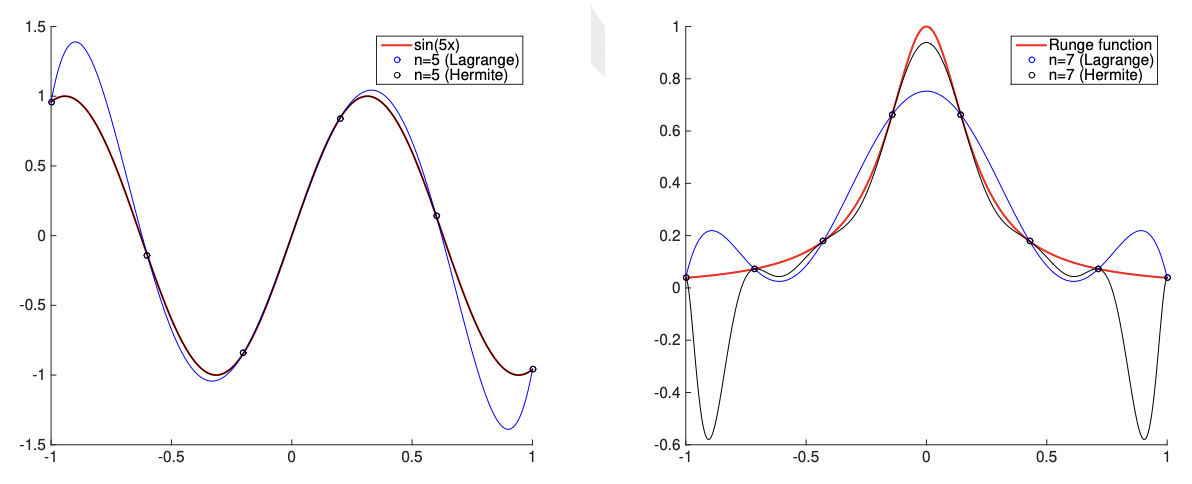
\includegraphics[width=\textwidth]{figures/fig-21.png}
\end{center}